\documentclass[11pt,a4paper]{article}
\usepackage{amsmath}
\usepackage{amssymb}
\usepackage{fullpage}
\usepackage{graphicx}
\usepackage[colorlinks=true, linkcolor=blue]{hyperref}

\newcommand{\argmin}{\operatornamewithlimits{arg\,min}}
\renewcommand{\arraystretch}{1.15} % line spacing in tabular

\begin{document}
\title{Improving Image Understanding with Concept Graph}
\author{Libo Yin\\The Australian National University}
\maketitle
\section{The Original HEX Model}
\subsection{Structure}

The original HEX model \cite{deng2014large} is an extension of the baseline flat multiclass classification model. There are two types of multiclass classification: exclusive, where the classifier predicts exactly one out of all possible states to be true; and independent, where each state is predicted true or false independently. HEX finds a balance between these two ends of the spectrum. It models the hierarchical and exclusive relationship between concepts, extended by their hypernyms, with a semantic graphical model. Each node in this graphical model corresponds to a concept in the extended concept space being true or false. States of neighbouring nodes are constrained in that if $a$ is a hypernym of $b$, then is not allowed that $a=0,\ b=1$; and if $a$ and $b$ are exclusive, then they cannot both be true. HEX model classifies an image into a hierarchy that satisfies the above semantic consistency. A simple HEX graph is shown in \hyperref[fig:naive]{figure~\ref{fig:naive}}.
\begin{figure}[htbp]
\centering
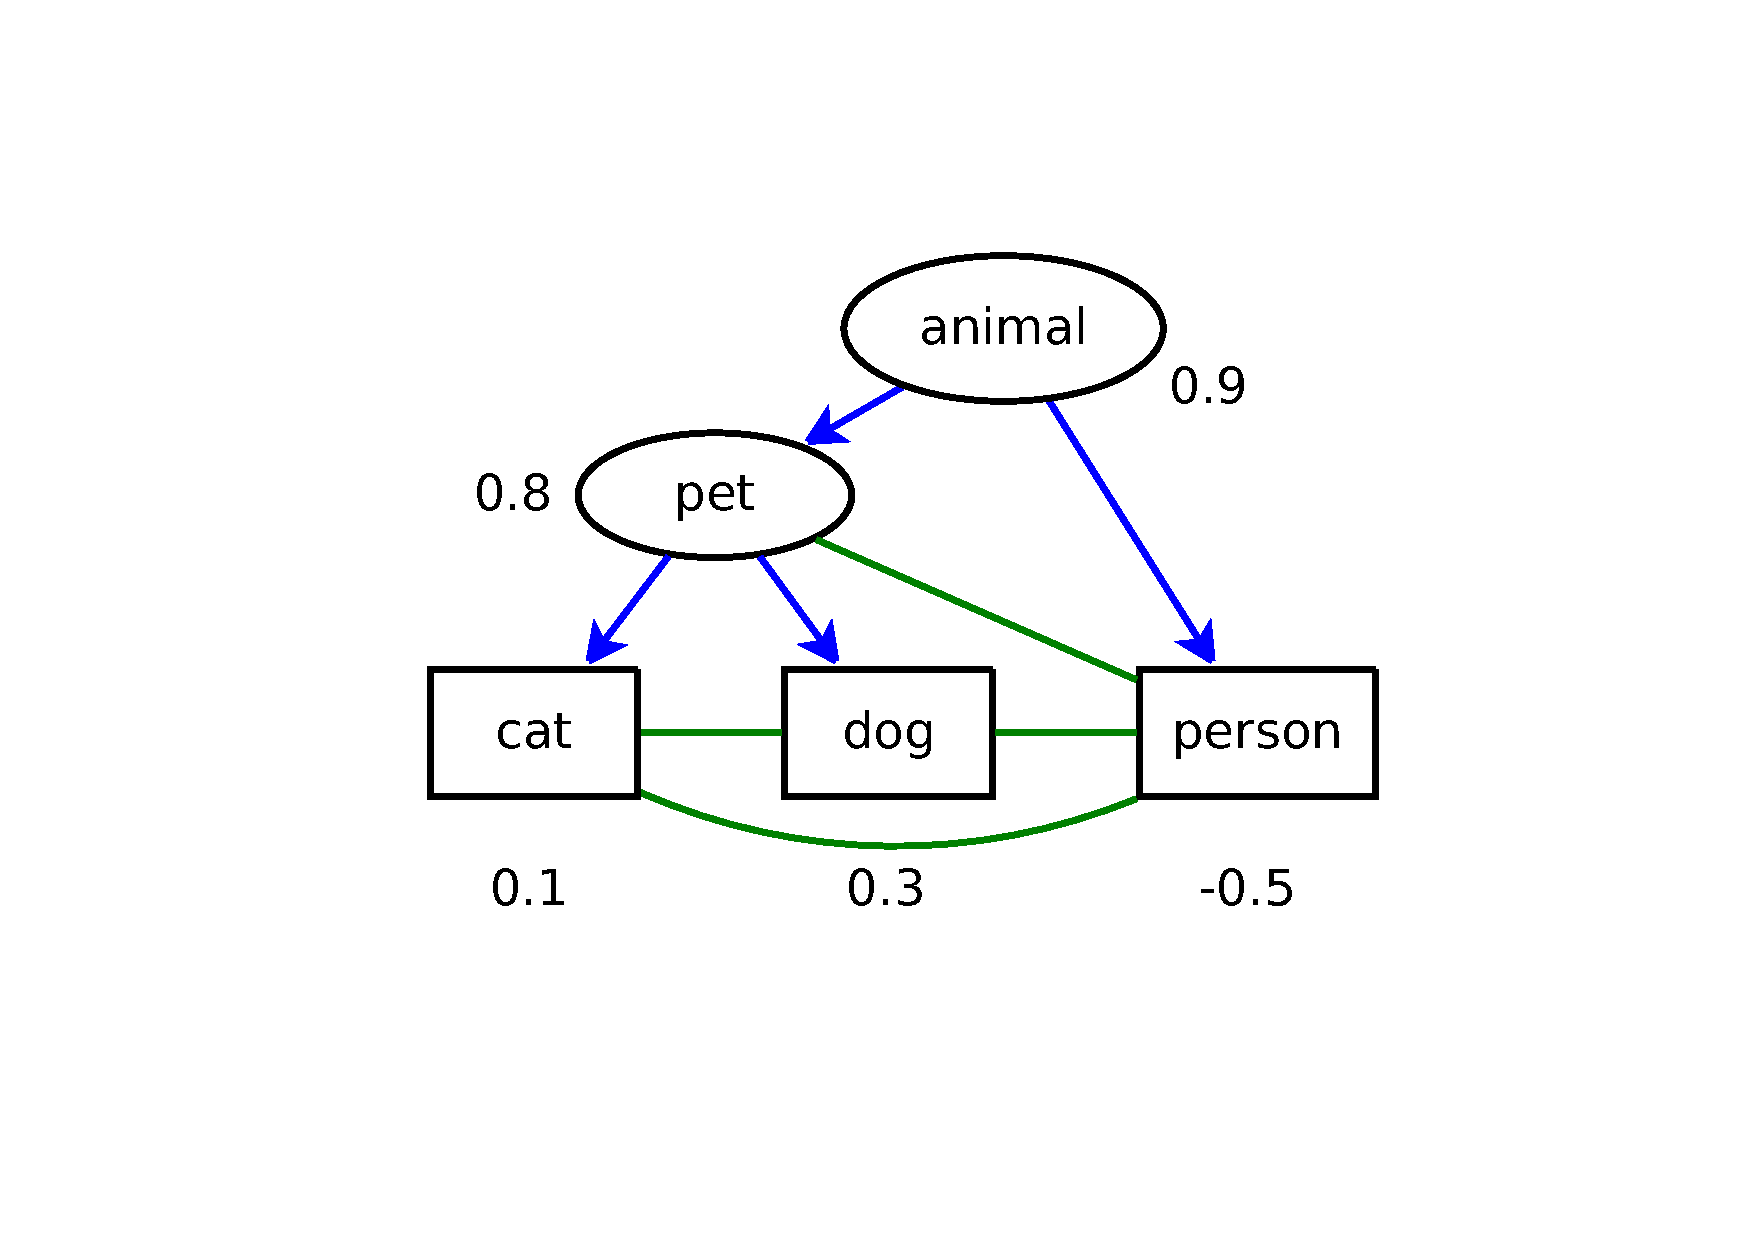
\includegraphics[scale=0.5]{naive.pdf}
\caption{A simple HEX graph with three nodes in the original concept space (in rectangles) and their hypernyms (in ellipsoids). Directed (blue) edges denote semantical hierarchy: $(a\rightarrow b)$ if $a$ is a hypernym of $b$ according to WordNet; and undirected edges (green) denote exclusion. Since exclusive relationship is not covered by WordNet, the exclusive subgraph is initialized greedily: two concepts are exclusive unless they share a common descendant in the hierarchical subgraph. Note that: 1. Concepts in the original concept space are mutually exclusive. 2. The hierarchical subgraph is in general a DAG rather than a tree.}
\label{fig:naive}
\end{figure}

Denoting the set of vertices by $V$, the set of hierarchical edges by $E_h$, and the set of exclusive edges by $E_e$, the joint assignment $y\in\{0,1\}^V$ can be defined as a CRF:
\begin{equation}
\tilde{p}(y|x)=\prod_{i\in V}\exp\{f_i(x;w)I[y_i=1]\}I[y\text{ legal}]
\label{eqn:naive}
\end{equation}

where unary input $f_i(x;w)$ is the confidence on concept $i$, predicted by an arbitrary underlying classifier\footnote{According to \cite{deng2014large}. It shall be explained in \hyperref[sec:observ]{section~\ref{sec:observ}} that the choice of underlying unary classifier is actually not arbitrary.}. Local semantic constraints on hierarchical and exclusive edges is formalised by
\begin{equation}
I[y\text{ legal}]=\prod_{(v_i,v_j)\in E_h}I[(y_i,y_j)\neq(0,1)]\prod_{(v_i,v_j)\in E_e}I[(y_i,y_j)\neq(1,1)]
\label{eqn:legal}
\end{equation}

Thanks to these semantic constraints, the state space of a HEX graph is significantly smaller than independent multiclass classification on the same concept space. For example, with local confidence given beside each node in \hyperref[fig:naive]{figure~\ref{fig:naive}}, the valid states of the HEX graph and their respective potentials are listed in \hyperref[tab:naive]{table~\ref{tab:naive}}:

\begin{table}[htbp]
\centering
\begin{tabular}{r|l}
state & $\tilde{p}(y|x)$\\
\hline
$\varnothing$ & $\exp(0)$\\
\{animal\} & $\exp(0.9)$\\
\{animal, pet\} & $\exp(0.9+0.8)$\\
\{animal, person\} & $\exp(0.9-0.5)$\\
\{animal, pet, cat\} & $\exp(0.9+0.8+0.1)$\\
\{animal, pet, dog\} & $\exp(0.9+0.8+0.3)$
\end{tabular}
\caption{Valid states of the HEX graph in \hyperref[fig:naive]{figure~\ref{fig:naive}} and their respective potentials. In this example, the HEX model predicts \{animal, pet, dog\}.}
\label{tab:naive}
\end{table}

Finally, an important assumption of \cite{deng2014large} is that mechanical Turks tend to label an image to more general concepts. For example, an image of a yellow Labrador may be labelled to ``dog''. Such behaviour is modelled by randomly relabelling an image to its immediate parents. As will be shown in \hyperref[sec:exp1]{section~\ref{sec:exp1}}, the higher the relabelling rate is, the larger is the advantage of the HEX model compared to the softmax baseline.

\subsection{Observations}
\label{sec:observ}

Note that a valid state does not have to have an active node in the original concept space. (Actually, it does not have to have an active node at all, as $\varnothing$ is a valid state according to \hyperref[eqn:legal]{(\ref{eqn:legal})}.) This allows an image to be classified to abstract concepts when the classifier is not confident enough to classify to a more concrete one. This is by no doubt a desirable feature for deployment. However, since all images are labelled in the original concept space of the dataset, classifying to the extended concept space makes performance evaluation troublesome. This issue was not addressed in \cite{deng2014large}. In this work, accuracy is tested both in the extended concept space and the original one, by limiting the legal state space to states with an active bottom-level node in the hierarchical subgraph.

Also note that in \hyperref[tab:naive]{table~\ref{tab:naive}}, the competition between state \{animal, pet, cat\} and \{animal, pet, dog\} depends entirely on the confidence of node ``dog'' and ``cat''. However, to discriminate between \{animal, pet, dog\} and \{animal, person\} requires examining the confidence along different paths. From this example it is clear that, in the testing stage, confidence is passed down the hierarchy from abstract concepts to concrete ones. The other side of the same coin is that, during the training stage of the underlying unary classifier, nodes corresponding to abstract concepts receive more training data compared to their children. This can be seen as confidence being passed up in the hierarchy. Such bidirectional propagation of confidence explains the advantage of the HEX model under the realistic labelling assumption.

The third observation is a combined consequence of the greedy exclusion setup, as discussed in the caption of \hyperref[tab:naive]{table~\ref{tab:naive}}, and the greedy nature of the potential function \hyperref[eqn:naive]{(\ref{eqn:naive})}. The prerequisite for the original HEX model to work is that the decision boundary of $f_i(x;w)$ is zero for all $i$. This is not a problem in \cite{deng2014large}, where a convolutional neural network \cite{krizhevsky2012imagenet} is used as the underlying unary classifier. However, if a probabilistic classifier is used, in which case $f_i(x;w)\in[0,1]$ and the decision boudary is 0.5, then it is guaranteed that a bottom-level node will be activated (see \hyperref[sec:fail]{appendix~\ref{sec:fail}} for proof). This means that the effective state space size is reduced to the that of the original concept space. In other words, the HEX model will not be able to predict to an abstract concept. This defeats the purpose of HEX, although inference can be performed easily with brute force calculation of the potential function \hyperref[eqn:naive]{(\ref{eqn:naive})}.

Finally, listed below are two less important observations:
\begin{enumerate}
\item There are no learnable variables in this CRF. In other words, all learning is performed in the underlying unary classifier.
\item Mathematically, CRF requires $\forall y:\tilde{p}(y|x)>0$. However, computationally, assigning zero to $\tilde{p}(y|x)$ can be interpreted as assigning an infinitesimal value. Therefore, the above definition is computationally equivalent to a legitimate CRF.
\end{enumerate}

\subsection{Problems}
\label{sec:problem}

Consider the situation illustrated in \hyperref[fig:depth]{figure~\ref{fig:depth}}:
\begin{figure}[htbp]
\centering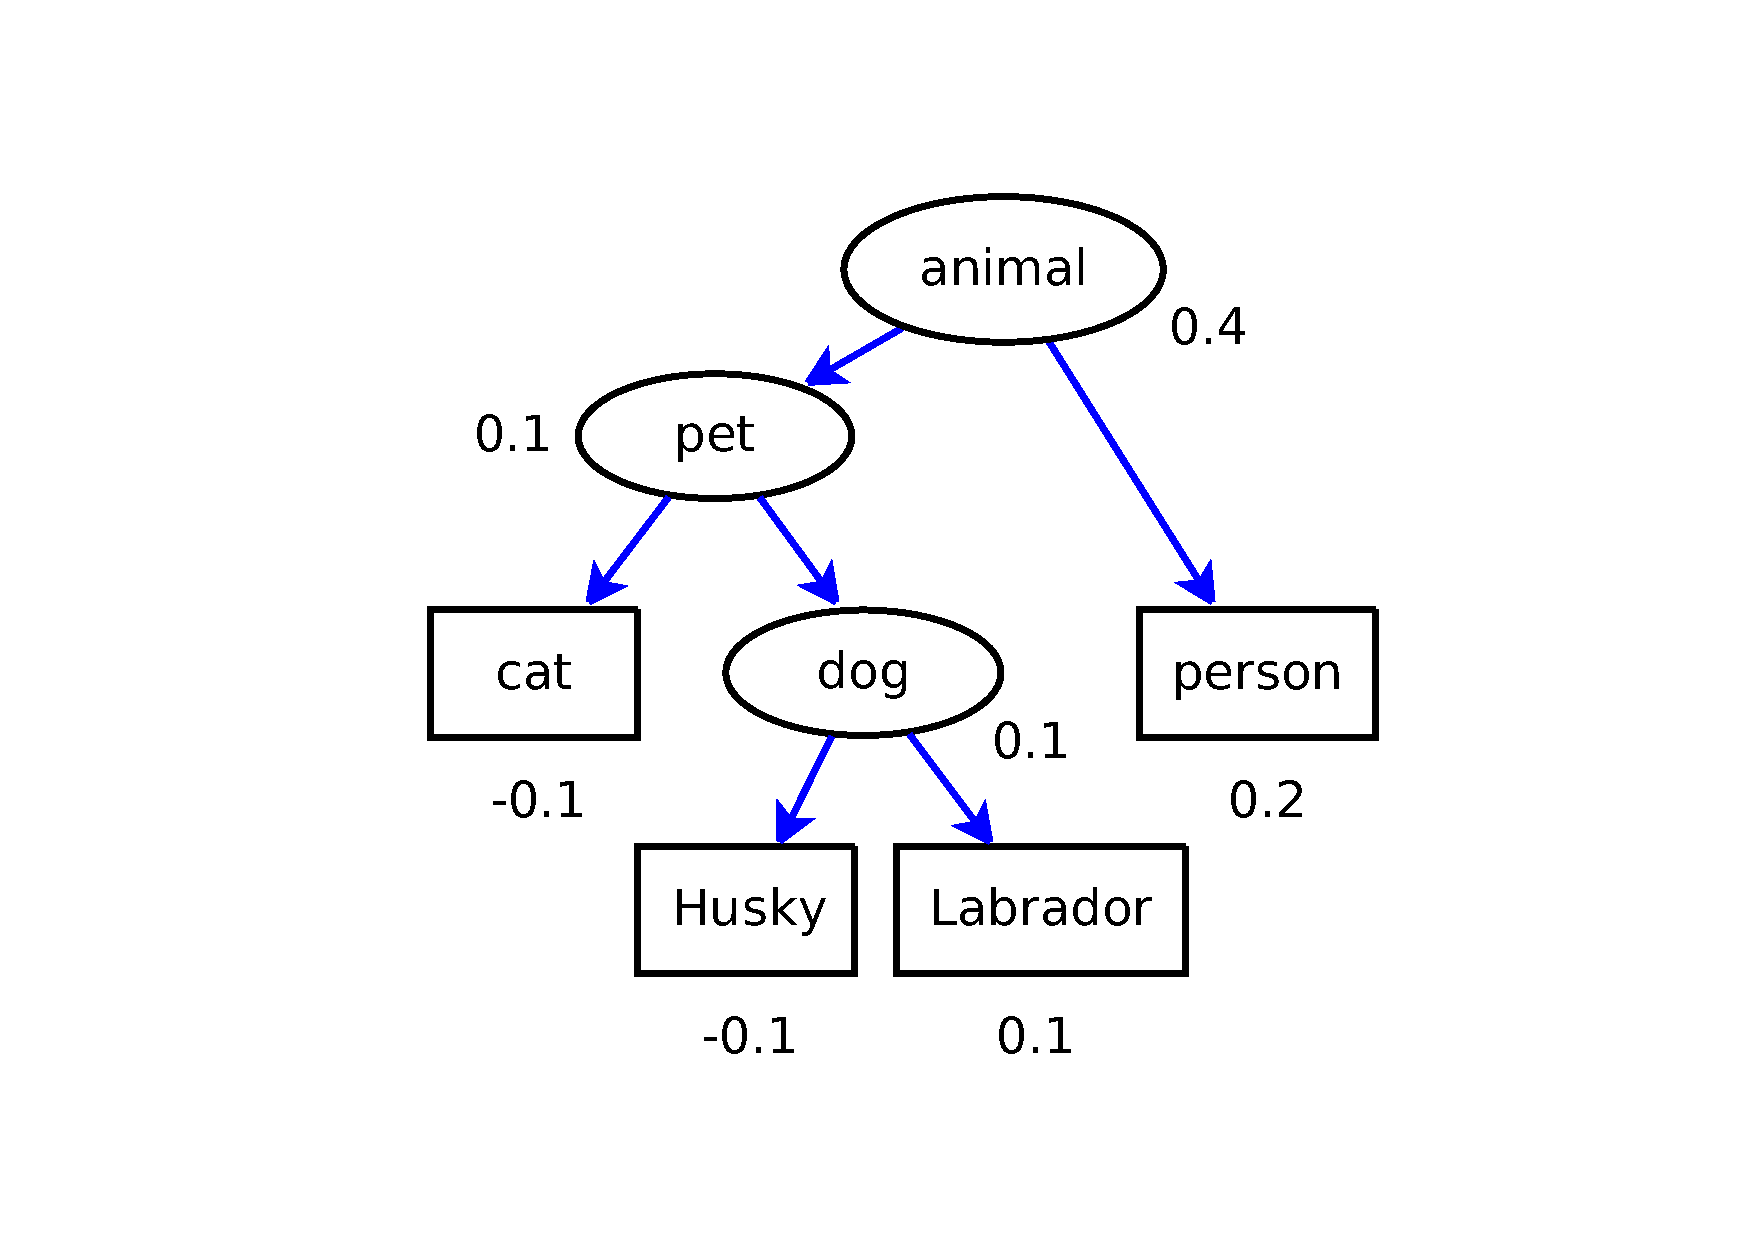
\includegraphics[scale=0.5]{depth.pdf}
\caption{Where a state with more active nodes of lower confidence wins over a state with fewer active nodes of higher confidence. Exclusive edges are omitted, as they do not carry further information once the state space has been calculated. The decision boundary of the underlying unary classifier is zero in this example.}
\label{fig:depth}
\end{figure}

Following the same logic as \hyperref[tab:naive]{table~\ref{tab:naive}}, the original HEX model predicts \{animal, pet, dog, Labrador\}. However, this is a result of more active nodes rather than active nodes of higher confidence. Intuitively, \{animal, person\} seems a better prediction. In addition, the two aforementioned assignments are very close to the decision boundary between them. It will be desirable if the model can make a prediction that is further from the decision boundary by taking into account the confidence of other nodes, especially those with unary predictions far from the decision boundary.

The second problem is a combined consequence of the realistic labelling assumption and using convolutional neural network as the underlying unary classifier. When the relabelling rate is high, most images are relabelled to their immediate parents. This does \emph{not} indicate that the unary classifiers for concepts in the original concept space receive fewer training samples, and are therefore undertrained; instead, it means that these classifiers receive incorrectly-labelled training data, where most images of concept X are labelled ``NOT X''. In such case, because CNN is trained as an independent multiclass classifier, those unary classifiers will pickup the imbalance, and simply predict ``false'' for any input images. The original HEX model cannot cope with such situation due to the greedy nature of potential function \hyperref[eqn:naive]{(\ref{eqn:naive})}, and will deactivate bottom-level concepts. This hypothesis will be confirmed in \hyperref[sec:exp1]{section~\ref{sec:exp1}}.

\clearpage
\section{Reimplementation}
\subsection{Dataset}
\label{sec:data}

The original HEX model is reimplemented as the baseline of this work. While \cite{deng2014large} used ILSVRC 2012 dataset for its rich structure in label space, this work employed PASCAL VOC 2012 \cite{pascal-voc-2012} for its simplicity (see \hyperref[fig:hex]{figure~\ref{fig:hex}} for the complete hierarchical subgraph). Note that the two datasets are designed for different tasks: ILSVRC is an exclusive multiclass classification problem, whereas PASCAL is an independent multiclass classification problem. To adapt to ILSVRC task 1, the train\,+\,val dataset of the PASCAL dataset is filtered through the following criteria:
\begin{enumerate}
\item If there is only one annotated object in the image, the image is labelled to that object.
\item If the largest annotated object in the image is more than twice as large as the second largest one, the image is labelled to its dominating object.
\end{enumerate}
\begin{figure}[p]
\centering
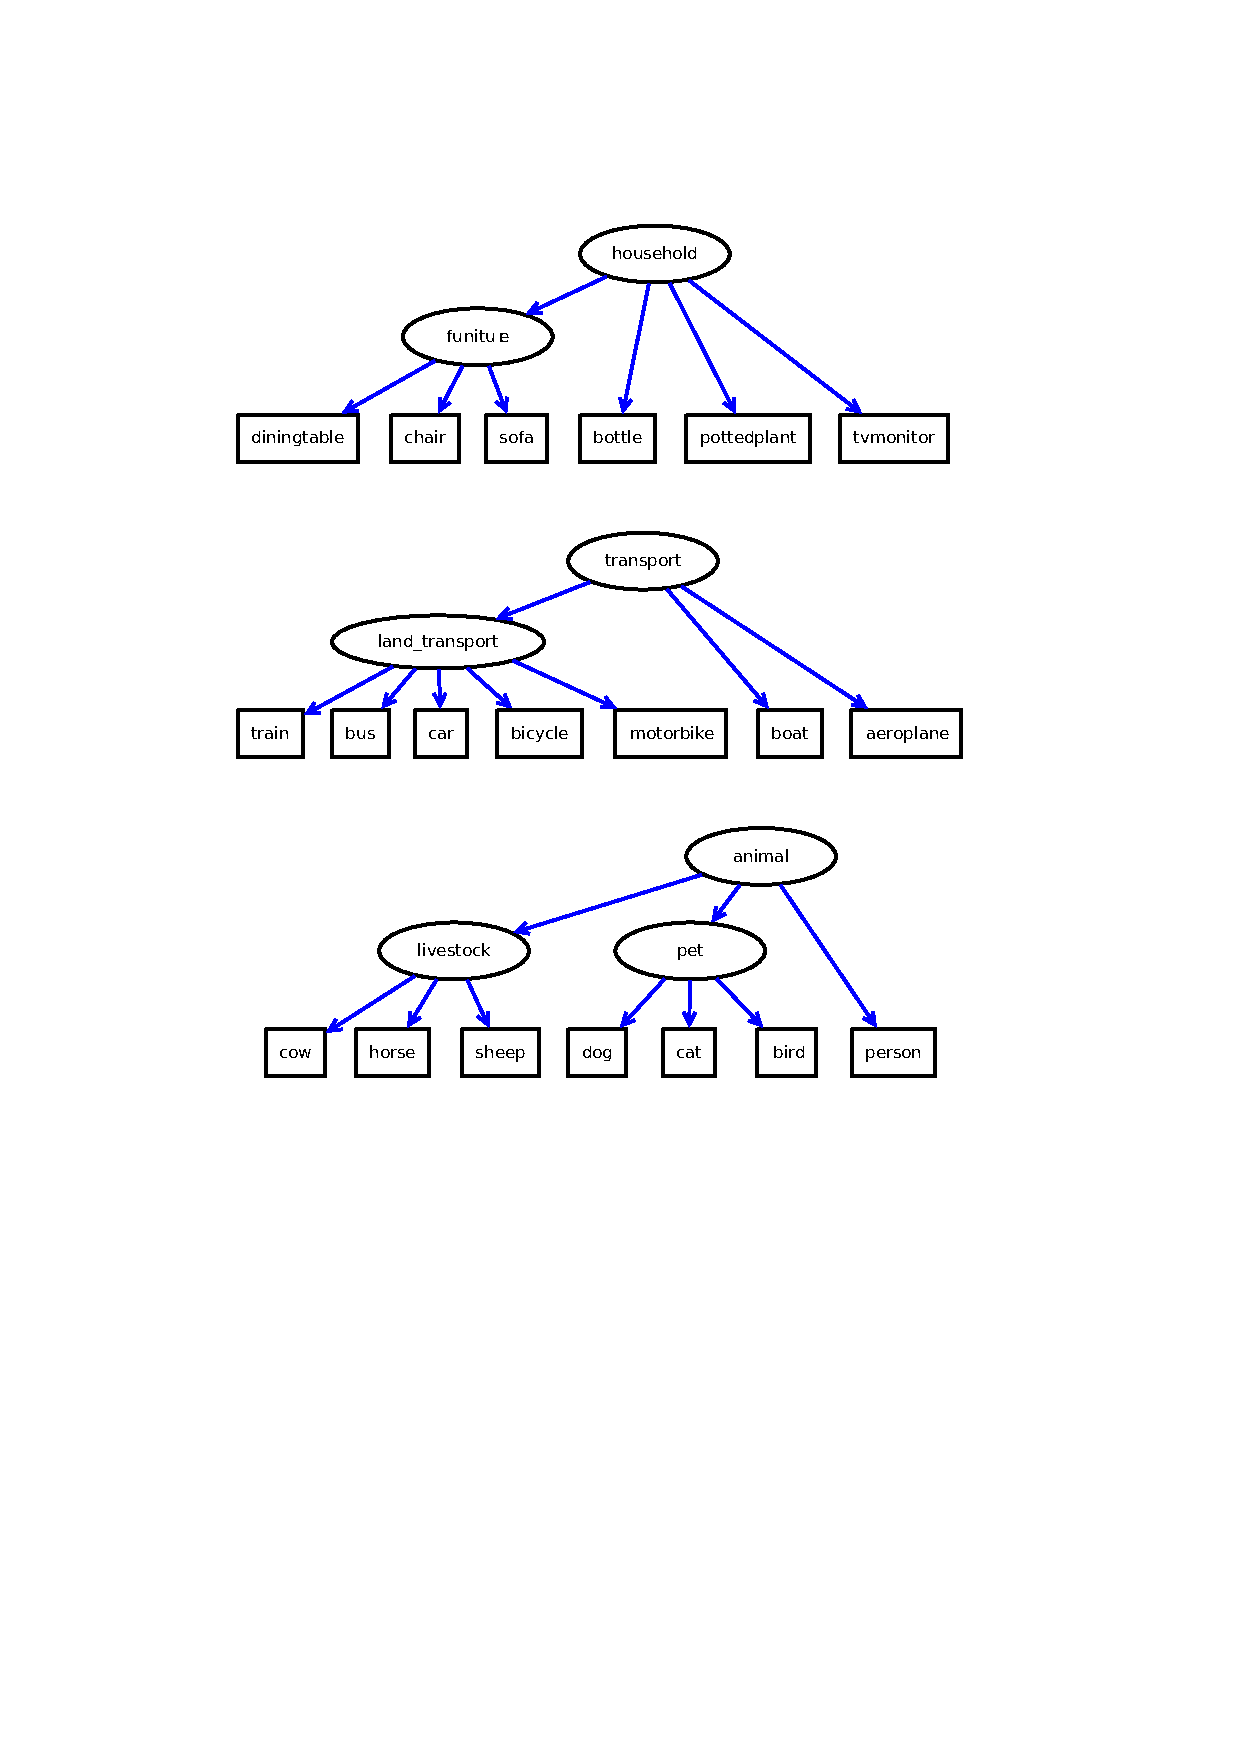
\includegraphics[scale=1.1]{full.pdf}
\caption{The PASCAL dataset has 20 concepts. In this work, these concepts are augmented by 7 of their hypernyms, creating a forest of three trees, 27 nodes, and 24 hierarchical edges. In comparison, the HEX graph for ImageNet contains 1000 nodes corresponding to the original concept space, and 840 nodes corresponding to their hypernyms.}
\label{fig:hex}
\end{figure}

Another major difference between ImageNet and PASCAL is that the former one is a balanced dataset, while the latter is unbalanced. For example, after filtering, there are 5324 images labelled as ``person'', whereas the second most frequent label ``dog'' has only 817 instances. To rebalance the dataset, 950 images of ``person'' are subsampled from the dataset.  After preprocessing, the dataset contains 8473 images in total. These images are then split 3:1:1 into train/validation/test set. The distribution of images across labels is illustrated in \hyperref[fig:distro]{figure~\ref{fig:distro}}.
\begin{figure}[htbp]
\centering
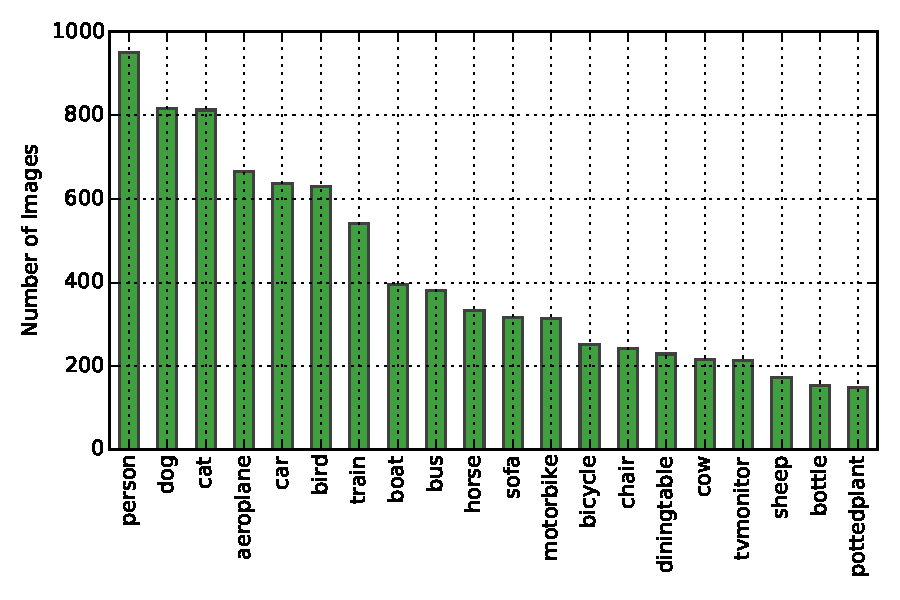
\includegraphics[scale=0.8]{distro.pdf}
\caption{Distribution of images according to labels, after preprocessing}
\label{fig:distro}
\end{figure}

\subsection{Algorithms}

For consistency with \cite{deng2014large}, the underlying unary classifier is based on \cite{krizhevsky2012imagenet} rather than the current state-of-the-art \cite{simonyan2014very}. The convolutional neural network is fine-tuned as an independent multiclass classifier with Caffe \cite{jia2014caffe}. Note that since the original HEX model has no learning part, it was built as a layer into the CNN, achieving end-to-end learning. In this work, CNN and CRF are implemented separately in order to test multiple variations of the HEX model with the same underlying unary classifier. The fine-tuning process finished within five hours on a GeForce GTX 470 graphical card.

A consequence of the simpler concept space is the change of inference algorithm. In \cite{deng2014large}, inference is performed by MAP loopy belief propagation on the maximally sparsified HEX graph, where the local state space of each clique is limited by semantic restrictions. In this work, thanks to the tiny state space of PASCAL, the inference is performed by calculating the potential function directly for each possible states in the global state space.

Finally, to guarantee that the benefit of the HEX model is consistent regardless of the underlying unary classifier, different variations of the HEX model are also paired with SVM as the underlying unary classifier. An array of 27 SVMs is trained, each corresponding to a node in the extended concept space. The SVM array accepts the output of the last-but-one layer of \cite{krizhevsky2012imagenet} as input, assuming that 4096 neurons provide sufficiently diverse and accurate feature responses without fine-tuning on the PASCAL dataset. The SVM array predicts either distance to decision boundaries or the probability of each concept being activated. The training process for the SVM array finished within ten hours without parallel training.

\subsection{Experiments}
\label{sec:exp1}
% original paper didn't give more than accuracy. more detailed analysis in exp2

\begin{table}[htbp]
\centering
\begin{tabular}{c|c|c|c|c}
Scheme & 0\% & 50\% & 90\% & 95\%\\
\hline
Baseline & 0.626(0.843) & 0.564(0.796) & 0.529(0.772) & 0.508(0.760)\\
Independent & N/A & 0.210(0.452) & 0.093(0.272) & 0.056(0.172)\\
HEX & N/A & 0.582(0.808) & 0.553(0.794) & 0.524(0.772)\\
\hline
Baseline & TODO & TODO & TODO & N/A\\
Independent & 0.171(0.733) & 0.004(0.625) & 0.000(0.172) & N/A\\
HEX & 0.657(0.777) & 0.318(0.719) & 0.000(0.477) & N/A
\end{tabular}
\caption{Comparison of empirical result in \cite{deng2014large} with reimplementation. Due to smaller dataset, 95\% relabelling rate was not attempted in this work. The result analysis of the original paper only provided accuracy. In this work, more detailed analysis is provided in \hyperref[sec:exp2]{section~\ref{sec:exp2}}}
\end{table}

\begin{table}[htbp]
\centering
\begin{tabular}{r|c|c|c}
 & 0\% & 50\% & 90\%\\
\hline
diningtable & $0.4285\pm0.3011$ & $0.2490\pm0.2288$ & $0.0108\pm0.0116$\\
furniture & $0.6976\pm0.3298$ & $0.7524\pm0.2784$ & $0.7330\pm0.3065$\\
household & $0.8431\pm0.2729$ & $0.8598\pm0.2490$ & $0.8590\pm0.2494$\\
\hline
dog & $0.7517\pm0.3424$ & $0.4533\pm0.2970$ & $0.0222\pm0.0209$\\
pet & $0.7971\pm0.3271$ & $0.7828\pm0.3327$ & $0.7832\pm0.3287$\\
animal & $0.9004\pm0.2301$ & $0.9005\pm0.2290$ & $0.8999\pm0.2322$
\end{tabular}
\caption{Under different relabelling rates, with fully trained CNN, the response on different concepts on the validation dataset, normalised with sigmoid function, and reported in $\mu\pm\sigma$. With 817 instances, label ``dog'' is a frequent label, whereas rare label ``diningtable'' has only 229 instances. Clearly, abstract concepts are not affected by relabelling rate, yet concrete ones drop from above the decision boundary to below. This experiment also shows that CNN learns highly abstract concepts accurately.}
\end{table}

\clearpage
\section{Improvements}

% Use all images to train the CNN, and images labelled to leaf nodes to train the CRF.

Based on the original HEX model, this work delivers improvements in three stages. In the first stage, the confidence on inactive nodes is taken into account, in addition to active ones. The resulting potential function is shown below:
\begin{equation}
\tilde{p}(y|x)=\prod_{i\in V}\exp\{f_i(x;w)I[y_i=1]+(1-f_i(x;w))I[y_i=0]\}I[y\text{ legal}]
\label{eqn:pn}
\end{equation}

This fix brings two benefits: First, the potential function considers the same number of nodes for different states, and therefore fixing the unnormalised depth problem mentioned in \hyperref[sec:problem]{section~\ref{sec:problem}}. Second, the potential function is able to refer to other nodes, benefiting from those that are far from the decision boundary. [std dev on cnn output on bottom-level nodes vs internal ones]

In the second stage, the unsure bottom-level nodes problem is solve by taking into account the pairwise terms, especially the hierarchical edges that connect the bottom-level nodes and their immediate parents. Two regularisation terms are also added to the potential function so that the contributions from nodes and edges are balanced.

In the third stage, Enable learning on unary and pairwise term weighting. With little confidence on the bottom layer classifiers, the problem is to attempt to classify to the bottom layers. However, in case the classifier really cannot make a decision, it should be allowed to stop at an intermediate layer. In order to do so, the CRF is trained with all images that are labelled to bottom-level concepts.

\[\theta=\argmin_\theta\left\{-\frac{C}{N}\log\prod_{(x,y)\in D}p_\theta(y|x)+\frac{1}{2}\|\theta\|^2\right\}\]

\begin{align*}
p_\theta(y|x)=\frac{1}{Z(x)}&\exp\left\{\frac{1}{|V|}\sum_{i\in V}w_i\big(x_i\cdot I[y_i=1]+(1-x_i)\cdot I[y_i=0]\big)\right\}\\
\cdot&\exp\left\{\frac{1}{|E|}\sum_{(i,j)\in E}t_{ij}\cdot x_ix_j\cdot I[y_i=y_j=1]\right\}\cdot I[y\text{ legal}]
\end{align*}

\begin{align*}
\log p_\theta(y|x)&=\frac{1}{|V|}\sum_{i\in V}w_i(x_i\cdot I[y_i=1]+(1-x_i)\cdot I[y_i=0])\\
&\quad+\frac{1}{|E|}\sum_{(i,j)\in E}t_{ij}\cdot x_ix_j\cdot I[y_i=y_j=1]-\log\sum_{\hat{y}}\tilde{p}_\theta(\hat{y}|x)
\end{align*}

\begin{align*}
\nabla_\theta\log\prod_{(x,y)\in D}p_\theta(y|x)&=\begin{bmatrix}
\nabla_w\log\prod_{(x,y)\in D}p_\theta(y|x)\\ 
\nabla_t\log\prod_{(x,y)\in D}p_\theta(y|x)
\end{bmatrix}\\
&=\begin{bmatrix}
\sum_{(x,y)\in D}\nabla_w\log p_\theta(y|x)\\ 
\sum_{(x,y)\in D}\nabla_t\log p_\theta(y|x)
\end{bmatrix}
\end{align*}

\begin{align*}
\nabla_w\log p_\theta(y|x)&=\underbrace{\frac{1}{|V|}\Big[x_i\cdot I[y_i=1]+(1-x_i)\cdot I[y_i=0]\Big]_{i\in V}}_{\phi_u(x,y)}-\nabla_w\log\sum_{\hat{y}}\tilde{p}_\theta(\hat{y}|x)\\
&=\phi_u(x,y)-\sum_{\hat{y}}p_\theta(\hat{y}|x)\cdot\phi_u(x,\hat{y})
\end{align*}

\begin{align*}
\nabla_w\log\sum_{\hat{y}}\tilde{p}_\theta(\hat{y}|x)&=\frac{1}{\sum_{\hat{y}}\tilde{p}_\theta(\hat{y}|x)}\nabla_w\sum_{\hat{y}}\tilde{p}_\theta(\hat{y}|x)\\
&=\frac{1}{Z(x)}\sum_{\hat{y}}\nabla_w\exp\left\{\frac{1}{|V|}\sum_{i\in V}w_i\big(x_i\cdot I[y_i=1]+(1-x_i)\cdot I[y_i=0]\big)\right\}\\
&\quad\cdot\exp\left\{\frac{1}{|E|}\sum_{(i,j)\in E}t_{ij}\cdot x_ix_j\cdot I[y_i=y_j=1]\right\}\\
&=\frac{1}{Z(x)}\sum_{\hat{y}}\tilde{p}_\theta(\hat{y}|x)\cdot\frac{1}{|V|}\Big[x_i\cdot I[\hat{y}_i=1]+(1-x_i)\cdot I[\hat{y}_i=0]\Big]_{i\in V}\\
&=\sum_{\hat{y}}p_\theta(\hat{y}|x)\cdot\phi_u(x,\hat{y})
\end{align*}

\begin{align*}
\nabla_t\log p_\theta(y|x)&=\underbrace{\frac{1}{|E|}\Big[t_{ij}\cdot x_ix_j\cdot I[y_i=y_j=1]\Big]_{(i,j)\in E}}_{\phi_t(x,y)}-\nabla_t\log\sum_{\hat{y}}\tilde{p}_\theta(\hat{y}|x)\\
&=\phi_t(x,y)-\sum_{\hat{y}}p_\theta(\hat{y}|x)\cdot\phi_t(x,\hat{y})
\end{align*}

\begin{align*}
\nabla_t\log\sum_{\hat{y}}\tilde{p}_\theta(\hat{y}|x)&=\frac{1}{\sum_{\hat{y}}\tilde{p}_\theta(\hat{y}|x)}\nabla_t\sum_{\hat{y}}\tilde{p}_\theta(\hat{y}|x)\\
&=\frac{1}{Z(x)}\sum_{\hat{y}}\nabla_t\exp\left\{\frac{1}{|V|}\sum_{i\in V}w_i\big(x_i\cdot I[y_i=1]+(1-x_i)\cdot I[y_i=0]\big)\right\}\\
&\quad\cdot\exp\left\{\frac{1}{|E|}\sum_{(i,j)\in E}t_{ij}\cdot x_ix_j\cdot I[y_i=y_j=1]\right\}\\
&=\frac{1}{Z(x)}\sum_{\hat{y}}\tilde{p}_\theta(\hat{y}|x)\cdot\frac{1}{|E|}\Big[t_{ij}\cdot x_ix_j\cdot I[\hat{y}_i=\hat{y}_j=1]\Big]_{(i,j)\in E}\\
&=\sum_{\hat{y}}p_\theta(\hat{y}|x)\cdot\phi_t(x,\hat{y})
\end{align*}

\subsection{Experiments}
\label{sec:exp2}

\begin{table}[htbp]
\centering
\begin{tabular}{r|l}
Scheme & Setup\\
\hline
1 & Ignore structure\\
2 & Independent\\
3 & Original CRF\\
4 & Sigmoid + pn CRF\\
5 & Sigmoid + pn CRF with pairwise term\\
6 & Sigmoid + learnable CRF
\end{tabular}
\caption{Test schemes}
\end{table}

\begin{table}[htbp]
\centering
\begin{tabular}{r|l|l|l}
Scheme & 0\% & 50\% & 90\%\\
\hline
2 & 0.1716(0.7339) & 0.0047(0.6258) & 0.0000(0.1728)\\
3 & 0.6573(0.7779) & 0.3182(0.7193) & 0.0000(0.4774)\\
4 & 0.6579(0.7790) & 0.3182(0.7197) & 0.0000(0.5154)\\
5 & 0.6923(0.7969) & 0.4631(0.7470) & 0.0005(0.5908)\\
6 & 0.6882(0.7802) & 0.4643(0.6496) & 0.1454(0.3646)
\end{tabular}
\caption{complete(top1/top3). Signs of overtrainning of CRF on the training set, but the benefit soon takes over as relabelling rate grows.}
\end{table}

\begin{table}[htbp]
\centering
\begin{tabular}{r|l|l|l}
Scheme & 0\% & 50\% & 90\%\\
\hline
1 & TODO & TODO & TODO\\
2 & 0.7268(0.8889) & 0.6739(0.8705) & 0.3230(0.5385)\\
3 & 0.7209(0.8788) & 0.6852(0.8574) & 0.5029(0.7838)\\
4 & 0.7214(0.8622) & 0.6799(0.8337) & 0.5000(0.7850)\\
5 & 0.7238(0.7957) & 0.6252(0.7470) & 0.3129(0.5908)\\
\end{tabular}
\caption{limited(top1/top3). Scheme 6 only apply to the extended concept space. WHAT DOES IT SAY?}
\end{table}

Stage 1: The problem is that, as discussed in \hyperref[sec:data]{section~\ref{sec:data}}... so the pnHEX model holds back conservatively?

Stage 3: It has been noticed that some weights are set to zero by optimisation.

\clearpage
\section{Discussions}
\subsection{Relationship to Probabilistic HEX}

Afte the ECCV 14 paper, the original authors extended HEX to pHEX by relaxing 0/1 hard constraints to $u\in(0,1)$, and turning the HEX graph into an Ising model \cite{ding2015probabilistic}. pHEX managed to beat HEX by [TODO]. However, the crucial $u$ is chosen by cross-validation, and it still applies to all constraints in the graph. In addition, pHEX require a long time to train, although still much shorter than training the underlying CNN. Also, it uses the same potential function as original HEX. Compared to pHEX, this work focuses on using a more flexible potential function. In term of running time, these two works are not directly comparable since this work is not scalable.

\subsection{Scalability}

Scalable until stage 2. Stage 3 is not scalable due to the brute force calculation of partition function. [download large hex graph from pHEX paper, see state space size]

\clearpage
\appendix
\section{Original HEX Fails with Positive Unary Inputs}
\label{sec:fail}

Denote the set of active nodes in a state by $\mathcal{S}$. Then there are three cases:
\begin{enumerate}
\item Assume there exists exactly one node $t$, such that $\forall s\in\mathcal{S}:s\rightarrow t$. In other words, $t$ is the only node among all active ones with no out-edges. If $t$ has children, then labelling any of them as true improves \hyperref[eqn:naive]{(\ref{eqn:naive})}.
\item Assume there exists two active nodes with no out-edges. Denote them by $t_1$ and $t_2$. Then they must share a common descendant, as otherwise they would be connected by an exclusive edge.
\begin{enumerate}
\item If they share a common immediate child $c$, then labelling $c$ as true improves \hyperref[eqn:naive]{(\ref{eqn:naive})}.
\item If they only share a distant descendant, then the state of $t_1$ and $t_2$ are independent. The problem is thus equivalent to two case 1 in parallel.
\end{enumerate}
\item There exists more than two active nodes with no out-edges. then each pair of them must have a common descendant, and the case is equivalent to pairwise case 2.
\end{enumerate}
Hence, it is guaranteed that for positive unary inputs, the original HEX labels to a node in the original concept space.

\section{Attributed HEX}

In earlier stages of this project, one of the proposed directions was the joint analysis of concept and attributes. That is, for example, to classify an image of a yellow Labrador into ``animal, pet, dog, yellow, furry'', etc. An example HEX graph is shown as follows:

While the training data is provided by aPascal \& aYahoo dataset \cite{farhadi2009describing}. [TODO: discuss dataset properties] The possibility of using CNN as feature extractor has been confirmed in \cite{razavian2014cnn}.

We only connected attributes to bottom-level concepts. In other words, the aHEX graph can be seen as a semantic part and an attribute part. Such design is for the sake of reducing loops in the aHEX graph. While junction-tree algorithm could potentially handle such a loopy graph during inference stage, the loops makes the graph very tricky to learn as a CRF. Similar design has been applied to pixel labelling problem such as [TODO: find references].

However, it was not the loops that caused such idea to be dropped. Under the same non-learning model, potential function is submodular, therefore such extension s trivial. Under the learnable CRF model, the aHEX graph can be learned part-wise: the semantic subgraph can be learned in the same way as discussed in [TODO: cross-ref learnable CRF], whereas for the attributes part, all bottom-level concepts can be grouped into a super-concept with 20 states (corresponding to 20 PASCAL labels), then the attribute graph becomes a tree, which is learnable[TODO: find references]. With such model, the inference is the same as an non-learning system, as the potential function for the attributed part still has a submodular structure.

\clearpage
\bibliographystyle{plain}
\bibliography{ref}
\end{document}